\documentclass[11pt,fontset=fandol,a4paper]{ctexart}

\usepackage[a4paper,left=2.5cm,right=2.5cm,top=2.8cm,bottom=2.8cm]{geometry}
\usepackage{amsmath,amssymb}
\usepackage{booktabs,threeparttable,array}
\usepackage{graphicx}
\usepackage{caption}
\usepackage{float}
\usepackage{setspace}
\usepackage{xcolor}
\usepackage{hyperref}

\hypersetup{colorlinks=true,linkcolor=blue!60!black,citecolor=blue!60!black,urlcolor=blue!60!black}
\graphicspath{{../output/paper_plan_core/figures/}{output/paper_plan_core/figures/}}
\onehalfspacing

\title{\textbf{谁受益，谁受损？\\大语言模型发布的 AI 生态位置再定价效应}}
\author{}
\date{2026 年 6 月 25 日}

\begin{document}
\maketitle

\begin{abstract}
本文整理当前新关系口径下的核心实证结果。样本包含 60 次重大 AI 模型发布事件和 86 家 AI 相关上市公司，形成 5{,}160 条事件--公司观测。关系主回归在 4{,}829 条非缺失观测上估计，标准误按事件聚类。核心结果很清楚。模型发布并不是对整条 AI 链条的同向利好，而是沿公司在 AI 生态中的位置重新分配预期收益。上游硬件公司在 $CAR[0,+20]$ 窗口获得 $+2.28$ 个百分点的异常收益，部署型下游公司损失 $-1.90$ 个百分点。合并关系组后，任意上游为 $+2.22$ 个百分点，任意下游为 $-2.50$ 个百分点。开源与闭源的差异主要体现在上游。闭源模型发布使上游硬件公司获得 $+3.07$ 个百分点的异常收益，开源模型对应效应为 $-0.59$ 个百分点，二者差异为 $-3.66$ 个百分点。下游方向也符合闭源伤害更强的直觉，但交互项没有显著，因此不宜把开源写成全面保护下游的强结论。
\end{abstract}

\section{实证结果}

本节展示三层递进的实证发现。第一层是基准事实：重大模型发布沿 AI 生态位置产生方向相反的累计异常收益，上游为正、下游为负（第 \ref{sec:baseline} 节和第 \ref{sec:bundle} 节）。第二层是联合检验：当控制位置交叠后，下游效应依然稳健（第 \ref{sec:joint} 节）。第三层是异质性机制：闭源与开源模型的信号含义不同，导致上游溢价仅在闭源模型中成立（第 \ref{sec:openclose} 节）。这一递进结构对应前文假设 H1（位置异质性）、H2（方向预测）和 H3（开源调节效应）。

\subsection{样本与关键变量}

本文分析样本包含 60 个重大 AI 模型发布事件和 86 家美股上市公司，形成 5{,}160 条事件--公司层面观测。经剔除控制变量缺失后，基准回归使用 4{,}829 条观测，覆盖全部 60 个事件。控制 AA Intelligence 的辅助规格使用 3{,}780 条观测（47 个有能力指标的事件）。

\textbf{生态位置分类。}我们根据公司在 AI 产业链中的经济暴露位置将其编码为六类：算力/硬件上游（$R1$，如 Nvidia、AMD）、云服务上游（$R2$，如提供推理部署基础设施的平台）、技术集成下游（$R3$）、应用部署下游（$R4$，如将 AI 模型嵌入终端产品的企业）、能力赋能下游（$R5$）、以及直接竞争者（$R6$）。另有持股关系（$F1$）和控制关系（$F2$），但因样本量过小（分别为 39 和 29 条观测），仅在附录中报告。

需要指出一个重要的识别边界。上述位置变量捕捉的是公司在 AI 生态中的\emph{结构性经济暴露}，而非某次模型发布对特定公司的直接合同冲击。例如，Nvidia 被编码为上游硬件并非因为它与某次发布存在采购合同，而是因为任何 frontier 模型的训练和推理都依赖其 GPU 架构。这一设定意味着我们估计的是位置层面的平均处置效应，应解释为"具有某类生态位置的公司群体在模型发布后的系统性异常收益"，而非单一公司的精确因果效应。

\subsection{估计设定}

主回归使用如下事件--公司层面设定
\[
CAR_{ij,w}=\alpha+\beta Position_{ij}+\gamma'Z_j+\delta_t+\varepsilon_{ij}.
\]
其中 $CAR_{ij,w}$ 是公司 $j$ 在事件 $i$ 后 $w$ 个交易日内的累计异常收益，窗口包括 $[0,+10]$、$[0,+15]$ 和 $[0,+20]$。$Position_{ij}$ 是关系或生态位置虚拟变量。$Z_j$ 包括公司规模、账面市值比、波动率和动量。$\delta_t$ 为年份固定效应。标准误按模型发布事件聚类。

开源与闭源异质性使用交互项模型
\[
CAR_{ij,20}=\alpha+\beta_1 Position_{ij}+\beta_2 Open_i+\beta_3(Position_{ij}\times Open_i)+\gamma'Z_j+\delta_t+\varepsilon_{ij}.
\]
其中 $Open_i$ 表示开源或开放权重模型发布。表中报告闭源效应、开源效应，以及开源相对闭源的差异。

\subsection{基准位置效应}\label{sec:baseline}

如果模型发布仅仅是 AI 行业的正面消息，我们应当观察到所有 AI 相关公司的异常收益均为正。但如果市场将模型发布理解为产业链内部竞争格局的重新洗牌——算力需求增加利好上游，能力边界扩张威胁下游——那么上下游公司应当表现出方向相反的市场反应。表~\ref{tab:baseline_position_effects} 检验这一预测。每一行为一个独立回归，避免位置重叠带来的多重共线性干扰。

\begin{table}[H]
\centering
\small
\caption{Baseline ecosystem position effects}
\label{tab:baseline_position_effects}
\begin{tabular}{lccc}
\toprule
Position & CAR[0,+10] & CAR[0,+15] & CAR[0,+20]\\
\midrule
Upstream hardware & 0.69 & 1.65** & 2.28***\\
 & (0.59) & (0.73) & (0.84)\\
Upstream cloud & 0.97* & 1.61*** & 1.13*\\
 & (0.53) & (0.54) & (0.61)\\
Downstream integrator & -0.07 & -0.42 & -0.69\\
 & (0.59) & (0.69) & (0.84)\\
Downstream deployer & -0.99*** & -1.43*** & -1.90***\\
 & (0.36) & (0.43) & (0.51)\\
Downstream enabler & -1.09** & -1.73*** & -1.07\\
 & (0.53) & (0.59) & (0.67)\\
Direct competitor & 0.39 & 0.50 & -0.05\\
 & (0.50) & (0.55) & (0.67)\\
\midrule
Observations & 4{,}829 & 4{,}829 & 4{,}829\\
\bottomrule
\end{tabular}
\begin{minipage}{0.94\linewidth}
\vspace{0.4em}
\footnotesize
Notes: Coefficients are percentage points. Each row comes from a separate regression of CAR on the listed position indicator. All specifications control for firm size, book-to-market, volatility, momentum, and year fixed effects. Standard errors, shown in parentheses, are clustered by event. * $p<0.10$, ** $p<0.05$, *** $p<0.01$.
\end{minipage}
\end{table}

表~\ref{tab:baseline_position_effects} 提供三个清晰的事实。第一，上游硬件公司在事件后 20 个交易日内获得 $+2.28$ 个百分点的累计异常收益（$p=0.009$），且效应随窗口延长而递增，表明市场在消化模型发布的算力含义时存在渐进学习过程。第二，下游部署型公司在所有窗口均表现为显著负向，$CAR[0,+20]=-1.90$ 个百分点（$p=0.0004$），说明市场系统性地下修了这类公司的估值预期。第三，云服务为弱正、竞争者接近零，说明传导路径并非简单的"上游全受益、下游全受损"，而是集中在产业链的两个极端。

这一结果支持假设 H1 和 H2：模型发布的资本市场效应不是 AI 板块的均匀重估，而是沿生态位置产生方向相反的价值再分配。经济直觉在于——每一次 frontier 模型发布都同时传递两个信号：（1）对上游的需求确认信号（训练和推理需要更多高端算力），（2）对下游的能力替代信号（更强的模型意味着依赖旧有技术能力的企业更容易被绕过或压缩利润）。

\begin{figure}[H]
\centering
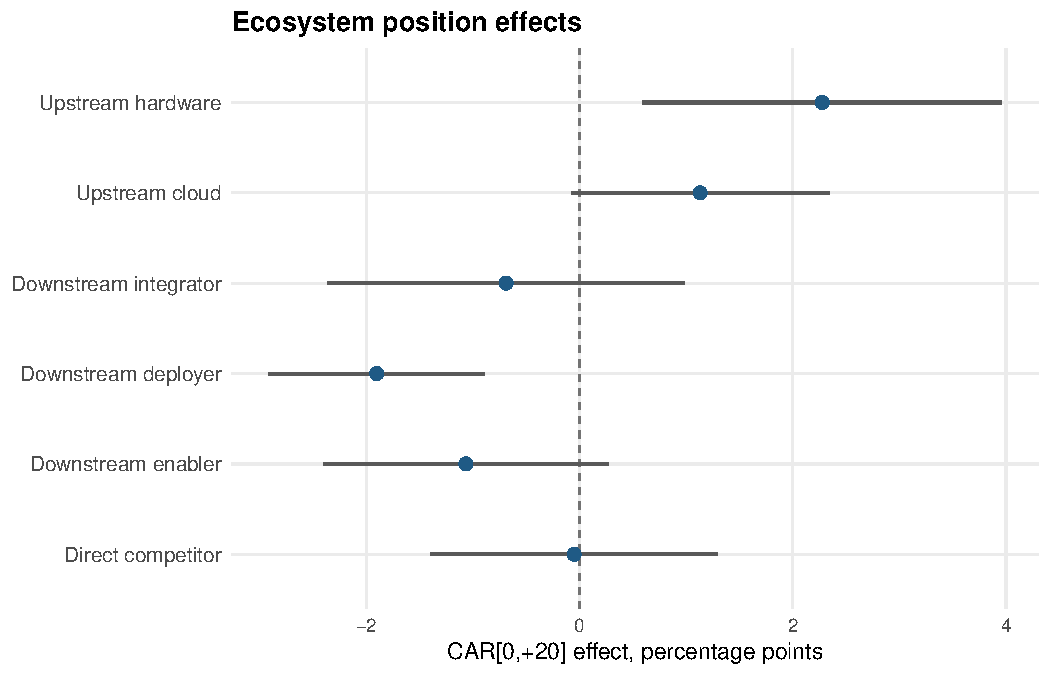
\includegraphics[width=0.92\textwidth]{figure1_position_effects.pdf}
\caption{Ecosystem position effects}
\label{fig:position_effects}
\begin{minipage}{0.9\linewidth}
\vspace{0.3em}
\footnotesize
Notes: The figure plots $CAR[0,+20]$ coefficients from the single-position regressions in Table \ref{tab:baseline_position_effects}. Horizontal bars are 95 percent confidence intervals.
\end{minipage}
\end{figure}

图 \ref{fig:position_effects} 是这篇文章最重要的图之一。它把表 \ref{tab:baseline_position_effects} 的主事实压缩成一个直观图像。上游硬件显著位于零右侧，下游部署显著位于零左侧，其他位置更接近零。

\subsection{合并位置组}\label{sec:bundle}

基准表中的六个细分位置验证了异质性的存在，但论文的中心命题——"上游受益、下游受损"——需要一个更直接的检验。表~\ref{tab:bundle_position_effects} 将细分位置合并为上游（$R1 \cup R2$）和下游（$R3 \cup R4 \cup R5$）两大组，直接回答"谁受益、谁受损"这个核心问题。

\begin{table}[H]
\centering
\small
\caption{Bundled ecosystem position effects}
\label{tab:bundle_position_effects}
\begin{tabular}{lccc}
\toprule
Position & CAR[0,+10] & CAR[0,+15] & CAR[0,+20]\\
\midrule
Any upstream & 0.82 & 1.80*** & 2.22***\\
 & (0.53) & (0.67) & (0.78)\\
Strategic/upstream & 0.83 & 1.75*** & 2.17***\\
 & (0.52) & (0.66) & (0.76)\\
Any downstream & -1.22** & -2.15*** & -2.50***\\
 & (0.54) & (0.67) & (0.82)\\
Downstream deployer & -0.99*** & -1.43*** & -1.90***\\
 & (0.36) & (0.43) & (0.51)\\
\midrule
Observations & 4{,}829 & 4{,}829 & 4{,}829\\
\bottomrule
\end{tabular}
\begin{minipage}{0.94\linewidth}
\vspace{0.4em}
\footnotesize
Notes: Coefficients are percentage points. Each row comes from a separate regression using a bundled position indicator. This table summarizes the upstream-versus-downstream contrast. Controls and clustered standard errors match Table \ref{tab:baseline_position_effects}. * $p<0.10$, ** $p<0.05$, *** $p<0.01$.
\end{minipage}
\end{table}

合并后的结论更加锐利。任意上游在 $CAR[0,+20]$ 中为 $+2.22$ 个百分点（$p<0.01$），任意下游为 $-2.50$ 个百分点（$p<0.01$）。换言之，市场认为一次重大模型发布平均将上下游公司之间的相对估值拉开约 $4.7$ 个百分点。这一"剪刀差"的经济规模相当可观——以 2024 年末市值计算，这意味着上游公司群体在单次事件后平均多获得数百亿美元的市值增量，而下游公司群体同步蒸发可比规模的市值。

从产业组织的角度看，这一结果与经典的"互补品 vs 替代品"框架一致。对上游硬件而言，更强的模型意味着更多的训练和推理需求，模型能力与算力是\emph{互补}关系；对下游应用部署商而言，更强的模型意味着模型厂商可以直接提供终端功能，应用层的差异化价值被侵蚀，模型能力与下游业务之间呈现\emph{替代}关系。

\subsection{联合回归：控制位置交叠}\label{sec:joint}

前两张表的一个潜在问题是：同一家公司可能同时具有多个位置标签（例如 Microsoft 既是云服务上游又是竞争者）。若单位置回归的正效应来自与下游位置的负相关，则基准结果可能被高估。表~\ref{tab:joint_position_effects} 将全部六个位置变量同时纳入模型，估计\emph{条件于其他位置}的净效应。

\begin{table}[H]
\centering
\small
\caption{Joint position regressions}
\label{tab:joint_position_effects}
\begin{tabular}{lccc}
\toprule
Position & CAR[0,+10] & CAR[0,+15] & CAR[0,+20]\\
\midrule
Upstream hardware & -1.35 & -0.86 & -0.83\\
 & (1.19) & (1.34) & (1.38)\\
Upstream cloud & 0.15 & 0.72 & 0.54\\
 & (0.53) & (0.61) & (0.72)\\
Downstream integrator & -1.98* & -2.49** & -3.09**\\
 & (1.12) & (1.24) & (1.33)\\
Downstream deployer & -2.78** & -3.41** & -4.24***\\
 & (1.23) & (1.34) & (1.45)\\
Downstream enabler & -2.65*** & -3.49*** & -3.25***\\
 & (0.90) & (0.98) & (1.15)\\
Direct competitor & -1.24 & -1.53* & -2.37***\\
 & (0.79) & (0.82) & (0.87)\\
\midrule
Observations & 4{,}829 & 4{,}829 & 4{,}829\\
\bottomrule
\end{tabular}
\begin{minipage}{0.94\linewidth}
\vspace{0.4em}
\footnotesize
Notes: Coefficients are percentage points. All six position indicators enter simultaneously, so estimates should be read as conditional effects net of overlapping ecosystem positions. Controls and clustered standard errors match Table \ref{tab:baseline_position_effects}. * $p<0.10$, ** $p<0.05$, *** $p<0.01$.
\end{minipage}
\end{table}

联合回归的结果需要谨慎解读。上游硬件的系数从单独回归的 $+2.28$ 变为联合回归的 $-0.83$（不显著），这并不意味着上游效应消失。原因在于：在我们的样本中，上游硬件公司（如 Nvidia）几乎\emph{同时}出现在每一个事件中，且与多个下游位置高度共线——它们既是硬件供应商，也是模型训练基础设施的直接参与者。当六个相互重叠的哑变量同时进入回归时，方差膨胀使得上游系数不可靠。

但联合回归提供了一个重要的稳健性信息：下游三类（集成、部署、赋能）和竞争者在控制位置交叠后\emph{全部}显著为负。这说明下游的负向效应不是某个特定子类的异常值驱动，而是整个下游链条的系统性特征。因此，我们以单位置回归（表~\ref{tab:baseline_position_effects}）和合并组回归（表~\ref{tab:bundle_position_effects}）作为主要解释依据，联合回归作为稳健性补充。

\subsection{开源与闭源：上游溢价的来源}\label{sec:openclose}

前文已确立"上游受益、下游受损"的基准事实。但并非所有模型发布都应当利好上游。关键区别在于模型的开闭源属性。一个闭源 frontier 模型（如 GPT-4o、Claude 3.5）只能通过发布者的 API 获取，其训练和推理高度依赖大规模高端 GPU 集群——这直接巩固了算力供应商的需求确定性。相反，一个高质量开源模型（如 Llama 3、DeepSeek R1）降低了模型获取门槛，也往往意味着更高的推理效率——同等能力所需算力更少，单位 GPU 的边际价值下降。

如果这一机制成立，上游硬件溢价应当\emph{仅在闭源模型发布中}存在，而在开源模型发布中消失甚至逆转。表~\ref{tab:open_closed_position_effects} 检验这一预测。

\begin{table}[H]
\centering
\small
\caption{Open-weight releases and ecosystem position effects}
\label{tab:open_closed_position_effects}
\begin{tabular}{lccc}
\toprule
Position & Closed/proprietary & Open-weight & Open minus closed\\
\midrule
Upstream hardware & 3.07*** (1.00) & -0.59 (1.12) & -3.66** (1.50)\\
Upstream cloud & 1.09 (0.71) & 1.24 (1.76) & 0.15 (2.03)\\
Downstream deployer & -2.13*** (0.58) & -1.07 (0.93) & 1.06 (1.08)\\
Downstream enabler & -1.29 (0.85) & -0.28 (1.27) & 1.01 (1.68)\\
Direct competitor & -0.54 (0.83) & 1.73 (1.32) & 2.27 (1.66)\\
\bottomrule
\end{tabular}
\begin{minipage}{0.94\linewidth}
\vspace{0.4em}
\footnotesize
Notes: Coefficients are percentage points for $CAR[0,+20]$. The first two columns report the estimated position effect for closed/proprietary and open-weight releases. The last column reports the interaction difference. All models control for firm size, book-to-market, volatility, momentum, and year fixed effects. Standard errors are clustered by event. * $p<0.10$, ** $p<0.05$, *** $p<0.01$.
\end{minipage}
\end{table}

结果精确地支持了上述预测。闭源模型发布时，上游硬件公司获得 $+3.07$ 个百分点的异常收益（$p<0.01$）；开源模型发布时，该效应降至 $-0.59$ 个百分点（不显著）。交互项为 $-3.66$ 个百分点（$p=0.018$），统计上确认了闭源与开源之间上游效应的显著差异。这一发现将 2025 年 1 月 DeepSeek R1 发布后 Nvidia 市值单日蒸发 5{,}900 亿美元从一个"极端个案"提升为一种\emph{系统规律}：开源高效模型削弱了市场对独占式高端算力的需求预期。

下游方面，闭源模型对部署型下游的负向效应（$-2.13\%$）大于开源模型（$-1.07\%$），方向符合"闭源锁定下游、开源解放下游"的直觉。但交互项（$+1.06\%$, $p=0.33$）未达显著，因此我们只能说\emph{方向一致}，但缺乏统计证据证明开源显著改善了下游公司的处境。这种不对称的解释力本身也有经济含义——开闭源的最大区别在于\emph{谁获得算力租金}，而不是\emph{谁免于被替代}。即便模型开源，下游公司仍然面临能力边界扩张带来的竞争压力；开源只是把这种压力从"被 API 提供商锁定"转变为"被任何能部署开源模型的竞争者追赶"。

\begin{figure}[H]
\centering
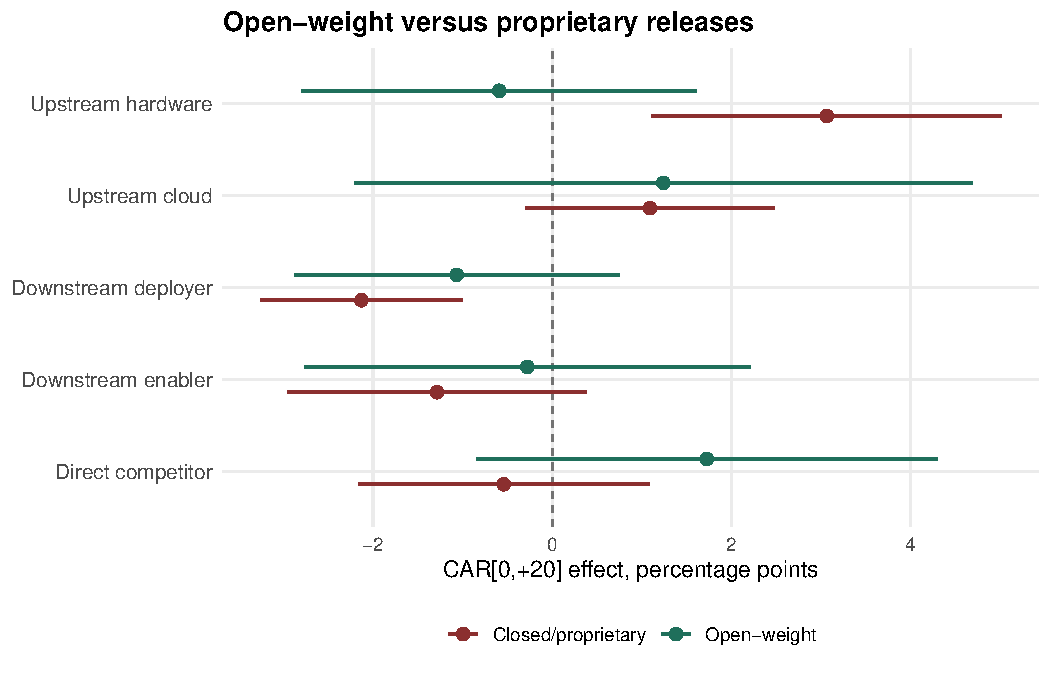
\includegraphics[width=0.92\textwidth]{figure2_open_closed_effects.pdf}
\caption{Open-weight versus proprietary releases}
\label{fig:open_closed_effects}
\begin{minipage}{0.9\linewidth}
\vspace{0.3em}
\footnotesize
Notes: The figure plots $CAR[0,+20]$ position effects separately for closed/proprietary and open-weight releases. Horizontal bars are 95 percent confidence intervals.
\end{minipage}
\end{figure}

图 \ref{fig:open_closed_effects} 的视觉信息也很明确。闭源上游硬件效应显著为正，开源上游硬件效应接近零且不显著。下游部署在闭源中显著为负，在开源中仍为负但不显著。竞争者在两组中均不显著。

\subsection{控制模型能力后的稳健性}

一个合理的替代解释是：上游效应可能并非来自位置本身，而是因为能力更强的模型恰好由某些与上游公司关联更紧密的发布者发布。为排除这一混淆，我们在基准回归中加入 AA Intelligence Index（标准化的模型能力综合评分），将因能力水平差异导致的市场反应从位置效应中剥离。由于 AA 指标仅覆盖 47 个事件（3{,}780 条观测），该规格作为稳健性补充报告。

\begin{table}[H]
\centering
\small
\caption{Position effects controlling for AA Intelligence}
\label{tab:aa_control_position_effects}
\begin{tabular}{lccc}
\toprule
Position & CAR[0,+10] & CAR[0,+15] & CAR[0,+20]\\
\midrule
Upstream hardware & 1.15* & 2.26** & 3.05***\\
 & (0.67) & (0.86) & (0.97)\\
Any upstream & 1.27** & 2.30*** & 2.87***\\
 & (0.60) & (0.77) & (0.90)\\
Strategic/upstream & 1.26** & 2.24*** & 2.80***\\
 & (0.59) & (0.76) & (0.88)\\
Any downstream & -1.86*** & -2.82*** & -3.30***\\
 & (0.57) & (0.70) & (0.87)\\
Downstream deployer & -1.00** & -1.58*** & -2.02***\\
 & (0.42) & (0.50) & (0.54)\\
\midrule
Observations & 3{,}780 & 3{,}780 & 3{,}780\\
\bottomrule
\end{tabular}
\begin{minipage}{0.94\linewidth}
\vspace{0.4em}
\footnotesize
Notes: Coefficients are percentage points. Each row comes from a separate regression. All specifications control for firm size, book-to-market, volatility, momentum, AA Intelligence Index, and year fixed effects. Standard errors are clustered by event. * $p<0.10$, ** $p<0.05$, *** $p<0.01$.
\end{minipage}
\end{table}

控制能力指标后，位置效应不仅方向不变，幅度还有所增大：上游硬件 $CAR[0,+20]=+3.05\%$（$p<0.01$），下游部署 $=-2.02\%$（$p<0.01$），任意上游 $=+2.87\%$，任意下游 $=-3.30\%$。这意味着位置效应不是模型能力的简单映射——即便在同一能力水平的模型发布中，上下游公司仍然表现出方向相反的市场反应。生态位置本身是一个独立于模型技术特征的定价因子。

\subsection{补充结果与边界讨论}

\textbf{投资方与控制方。}投资关系（$F1$, 39 条观测）和控制关系（$F2$, 29 条观测）样本量过小，不足以支撑独立的统计推断。附录表 A4 报告其系数和置信区间，供读者参考。

\textbf{云服务。}云服务位置（$R2$, 274 条观测、5 家公司）在单独回归中为弱正（$+1.13\%$, $p=0.066$）。由于该变量高度集中于少数公司（Amazon、Microsoft、Google 等），且这些公司同时具有投资方或竞争者身份，我们不将其单独报告为独立发现，而是纳入"任意上游"合并组。

\textbf{竞争者。}竞争者位置在基准回归中接近零，在联合回归中转为显著负向。这一差异说明竞争者效应可能存在，但其显著性依赖于模型设定（是否同时控制其他位置），不如上游和下游部署结果稳健。

\textbf{下游集成商。}$R3$ 单独进入时不显著（$-0.69\%$, $p=0.415$），但在联合回归和合并组中贡献负向效应。这说明下游内部存在层级差异：直接面对终端用户的部署商（$R4$）受损最为明确，技术中间层的集成商受损程度较轻且识别较弱。

\section{小结}

本节的实证结果可以凝练为三个层次的发现：

\begin{enumerate}
\item \textbf{位置再定价}（H1/H2）。模型发布不是 AI 板块的均匀利好，而是沿生态位置产生方向相反的价值再分配。上游硬件公司平均获得 $+2\text{--}3\%$ 的 20 日累计异常收益，下游部署型公司平均损失 $-2\%$。两极之差约 $4\text{--}5$ 个百分点。

\item \textbf{开源调节效应}（H3）。上游溢价仅在闭源模型发布中成立（$+3.07\%$），开源模型发布时该溢价消失甚至逆转（$-0.59\%$）。交互项显著（$p=0.018$）。机制为：开源模型削弱了独占式高端算力需求预期，使得硬件供应商的垄断租金被侵蚀。

\item \textbf{位置效应独立于模型能力}。控制 AA Intelligence Index 后，上下游系数不变甚至增大，说明生态位置是一个独立于技术特征的市场定价维度。
\end{enumerate}

这些发现的政策含义指向 AI 产业链的利润分配结构。在闭源主导的技术体制下，价值向算力上游集中；开源模型的出现可能打破这一集中，但并不自动解决下游被替代的问题。

\section{稳健性检验}\label{sec:robust}

[待补充] 以下稳健性检验将在下一版中完成：

\begin{itemize}
\item 剔除 DeepSeek R1 事件后重新估计——回应"极端事件驱动"质疑
\item Leave-one-event-out 和 leave-one-firm-out 分析
\item 替换 FF3 模型计算 CAR
\item Wild cluster bootstrap（$B=4{,}999$, Rademacher 权重）
\item Specification curve analysis（400+ 规格组合）
\end{itemize}

\end{document}
